Para uma \textit{Random Forest} decidi fazer o \textit{tuning} dos parâmetros \textit{Split Criterion} e \textit{Number of models}.

Para o primeiro parâmetro criei uma coluna com os valores \textit{Information Gain, Information Gain Ration} e \textit{Gini Index}.

\begin{figure}[H]
    \centering
    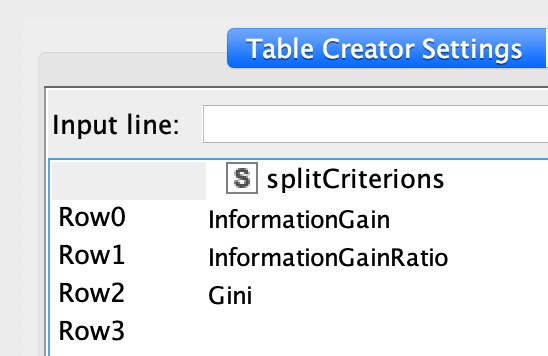
\includegraphics[scale=0.6]{Images/T5_b.png}
    \caption{Nodo Table Creator}
\end{figure}

Relativamente ao segundo parâmetro criei uma variável que itera entre os valores 100 e 200 (de 1 em 1). 

\begin{figure}[H]
    \centering
    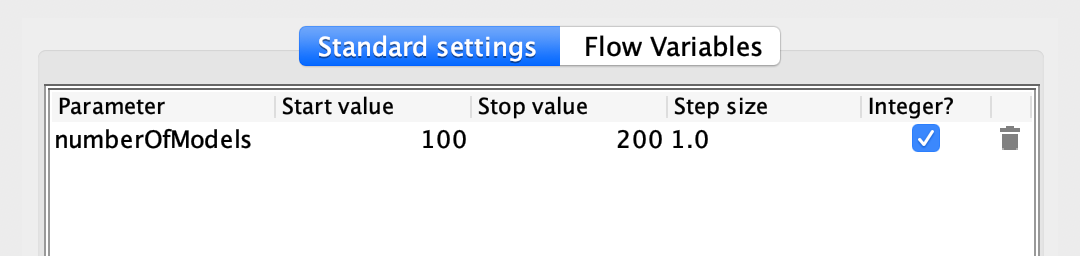
\includegraphics[scale=0.5]{Images/T5_c.png}
    \caption{Nodo Parameter Optimization Loop Start}
\end{figure}

\clearpage

No nodo \textit{Random Forest Learner}, na janela das \textit{Flow Variables}, associei as variáveis criadas anteriormente aos parâmetros do modelo.

\begin{figure}[H]
    \centering
    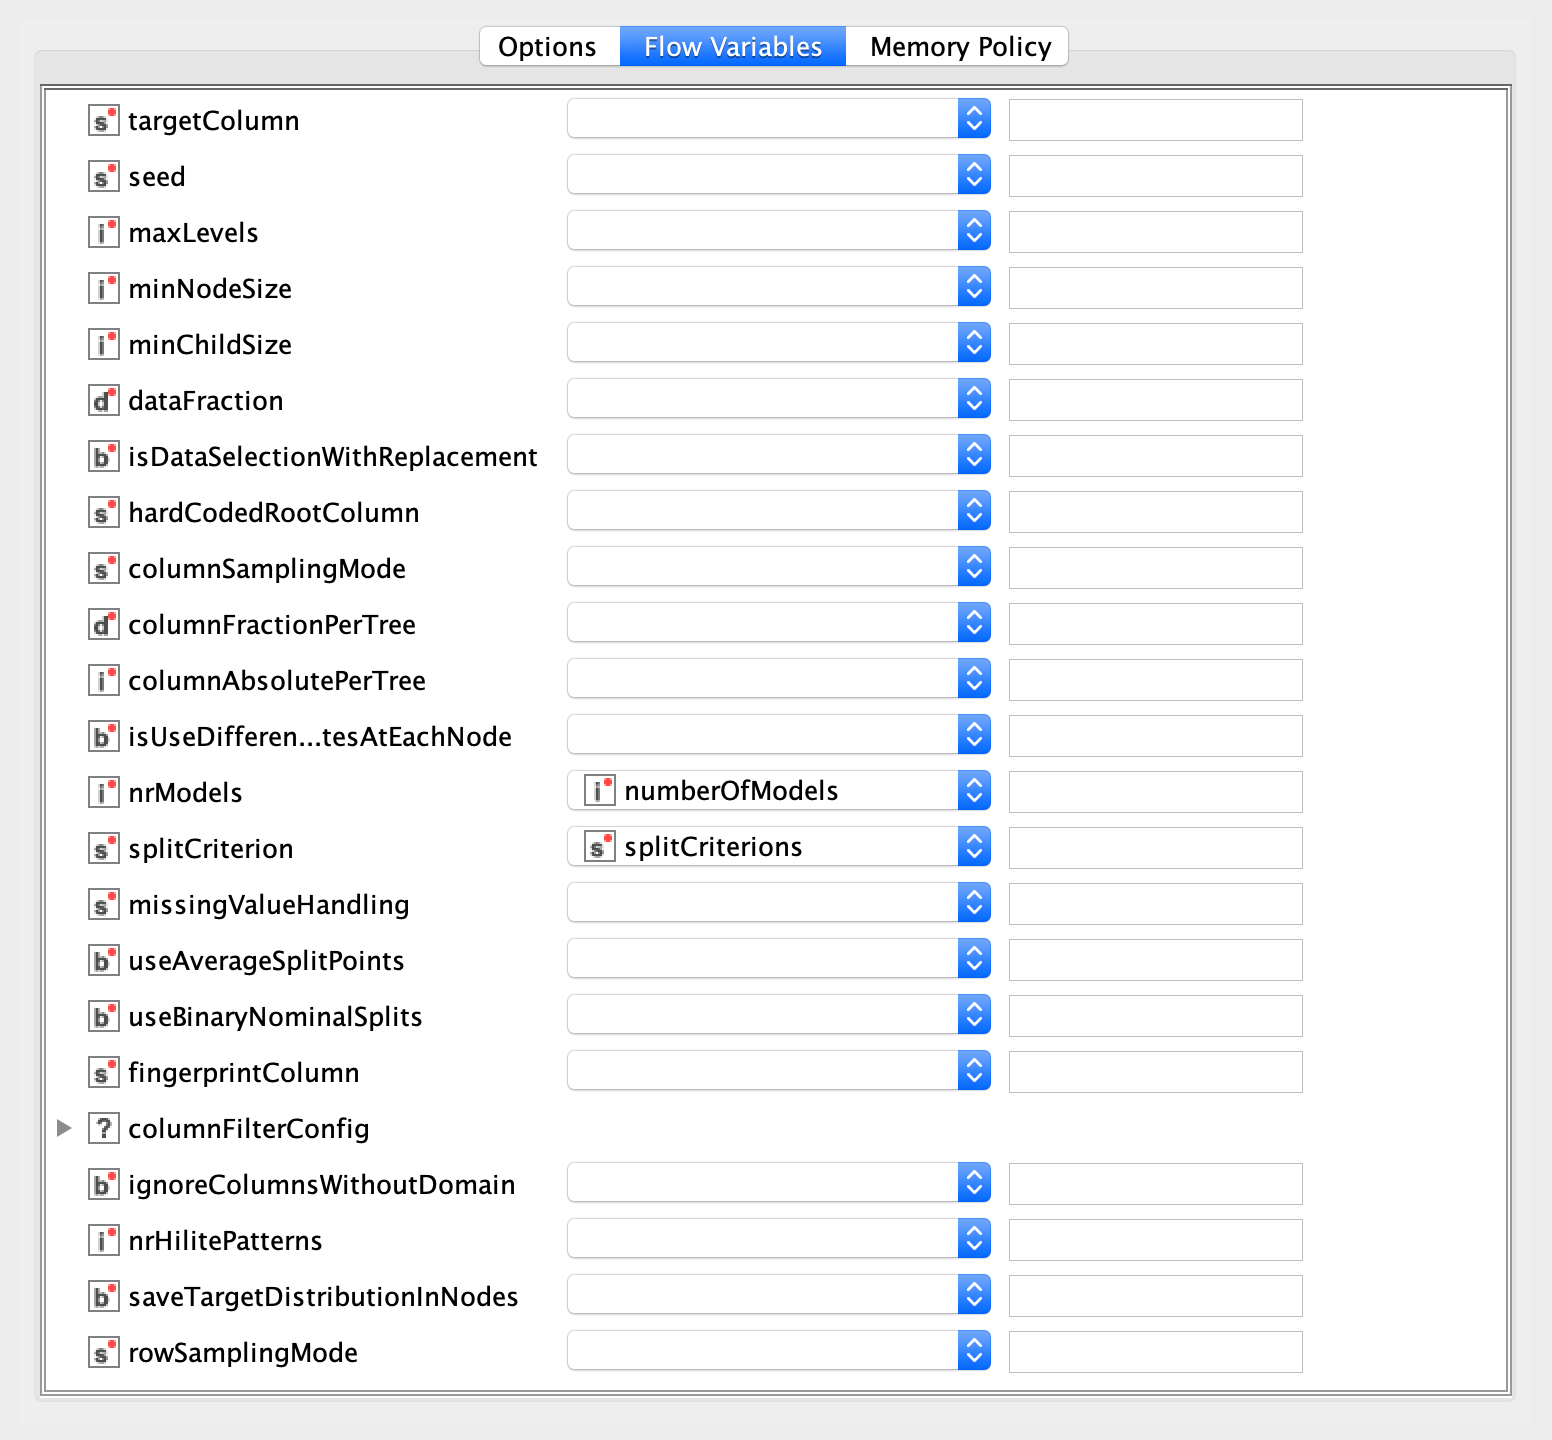
\includegraphics[scale=0.3]{Images/T5_d.png}
    \caption{Nodo Random Forest Learner}
\end{figure}

Por fim, obtive a seguinte combinação de parâmetros.

\begin{figure}[H]
    \centering
    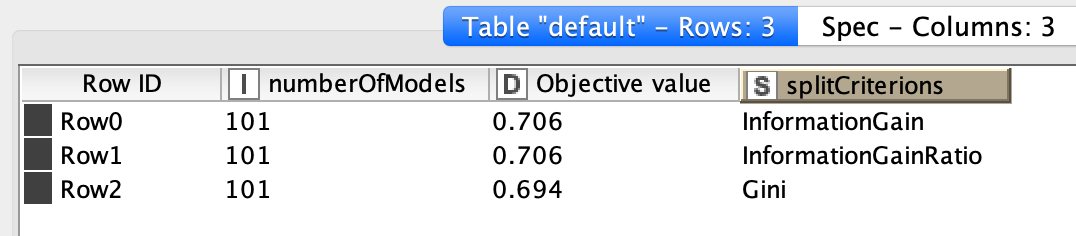
\includegraphics[scale=0.5]{Images/T5_e.png}
    \caption{Tabela resultante}
\end{figure}

O seguinte \textit{workflow} representa todos os passos realizados para esta tarefa.

\begin{figure}[H]
    \centering
    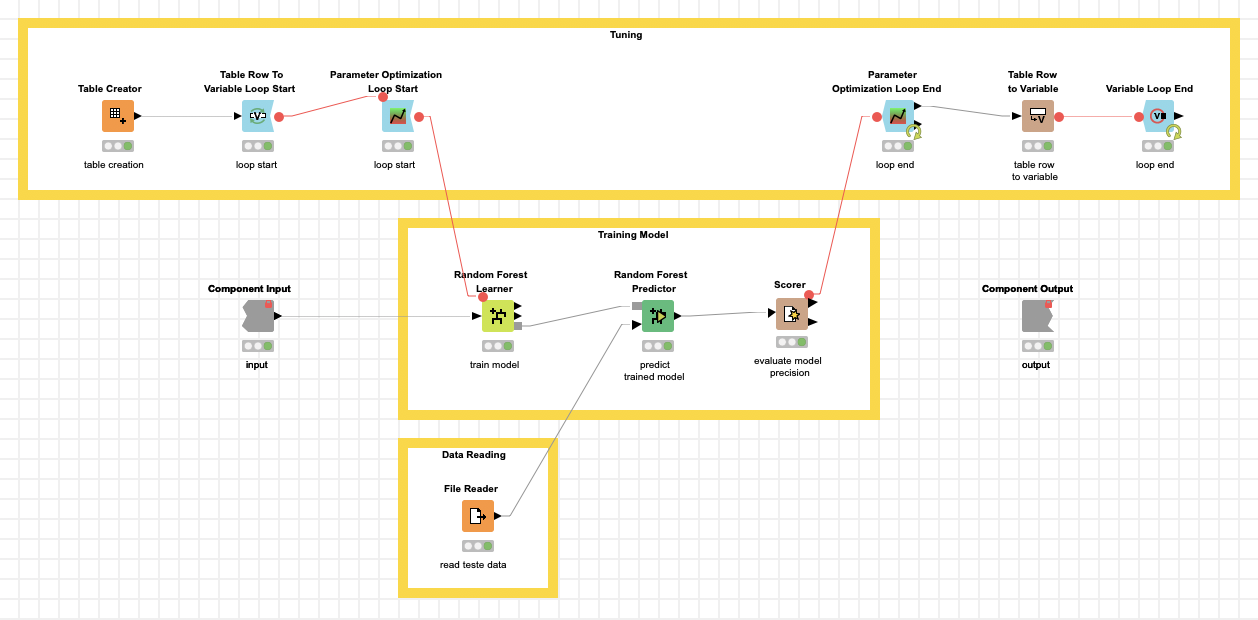
\includegraphics[scale=0.4]{Images/T5_a.png}
    \caption{Workflow}
\end{figure}